\documentclass{beamer}
%\usepackage[latin1]{inputenc}
\usetheme{Warsaw}
\title[Intro to Python: Week 8]{Introduction  to Python\\
                                Decorators -- Debugging -- Packages and Packaging}
\author{Christopher Barker}
\institute{UW Continuing Education / Isilon}
\date{August 22, 2012}

\usepackage{listings}
\usepackage{hyperref}

\begin{document}

% ---------------------------------------------
\begin{frame}
  \titlepage
\end{frame}

% ---------------------------------------------
\begin{frame}
\frametitle{Table of Contents}
%\tableofcontents[currentsection]
  \tableofcontents
\end{frame}


\section{Review/Questions}

% ---------------------------------------------
\begin{frame}[fragile]{Review of Previous Class}

{\Large Lightning talk today: Peter}

\begin{itemize}
    \item Some more OO
    \begin{itemize}
      \item Multiple inheritance / mix-ins
      \item Properties
      \item \verb|staticmethod| and \verb|classmethod|
      \item Special methods (``dunder'')
    \end{itemize}
      \item Iterators
      \item Generators
\end{itemize}

\end{frame}


% header
% ---------------------------------------------
\begin{frame}[fragile]{Homework review}

{\Large Who added some classes to some ``real'' code?}

{\Large 
\begin{itemize}
      \item Multiple inheritance / mix-ins ?
      \item Property ?
      \item \verb|staticmethod| or \verb|classmethod| ?
      \item Special methods ?
      \item Iterator or Generators ?
\end{itemize}
}
\end{frame}

\section{Decorators}

% ---------------------------------------------
\begin{frame}[fragile]{Decorators}

{\LARGE Decorators are wrappers around functions}

\vfill
{\LARGE They let you add code before and after the execution of a function}

\vfill
{\LARGE Creating a custom version of that function}

\end{frame} 

% ---------------------------------------------
\begin{frame}[fragile]{Decorators}

{\LARGE Syntax:}

\vfill
\begin{verbatim}
@logged
def add(a, b):
    """add() adds things"""
    return a + b
\end{verbatim}

\vfill
{\Large Demo and Motivation: \verb|basicmath.py| }

\vfill
PEP: \url{http://www.python.org/dev/peps/pep-0318/}

\end{frame} 

% ---------------------------------------------
\begin{frame}[fragile]{Decorators}

{\LARGE \verb|@| decorator operator is an abbreviation:}

\vfill
\begin{verbatim}
@f
def g:
    pass
\end{verbatim}

\vfill
same as

\vfill
\begin{verbatim}
def g:
    pass
g = f(g)
\end{verbatim}

\vfill
{\Large ``Syntactic Sugar'' -- but really quite nice}

\end{frame} 

% ---------------------------------------------
\begin{frame}[fragile]{Decorators}

{\LARGE demo:

\vfill
\begin{verbatim}
decorator.py
\end{verbatim}

}
\end{frame} 

% ---------------------------------------------
\begin{frame}[fragile]{Decorator  examples}

{\LARGE Examples from the stdlib:}

\vfill
{\Large Does this structure:}

\vfill
\begin{verbatim}
def g:
    pass
g = f(g)
\end{verbatim}

\vfill

{\Large look familiar from last class?}
\end{frame} 

% ---------------------------------------------
\begin{frame}[fragile]{Decorator examples}

{\LARGE \verb|staticmethod()|}

\vfill
\begin{verbatim}
class C(object):
    def add(a, b):
        return a + b
    add = staticmethod(add)
\end{verbatim}

\vfill

\end{frame} 

% ---------------------------------------------
\begin{frame}[fragile]{Decorator examples}

{\LARGE \verb|staticmethod()|}

\vfill
{\Large Decorator form:}
\begin{verbatim}
class C(object):
    @staticmethod
    def add(a, b):
        return a + b
\end{verbatim}

\vfill

{\LARGE ( and \verb|classmethod| )}
\end{frame} 

% ---------------------------------------------
\begin{frame}[fragile]{examples}

{\LARGE \verb|property()|}

\vfill
\begin{verbatim}
class C(object):
    def __init__(self):
        self._x = None
    def getx(self):
        return self._x
    def setx(self, value):
        self._x = value
    def delx(self):
        del self._x
    x = property(getx, setx, delx,
                 "I'm the 'x' property.")
\end{verbatim}

\vfill
becomes...
\end{frame} 

% ---------------------------------------------
\begin{frame}[fragile]{Decorator examples}

\begin{verbatim}
class C(object):
    def __init__(self):
        self._x = None
    @property
    def x(self):
        return self._x
    @x.setter
    def x(self, value):
        self._x = value
    @x.deleter
    def x(self):
        del self._x
\end{verbatim}

\vfill
Puts the info close to where it is used
\end{frame} 

% ---------------------------------------------
\begin{frame}[fragile]{examples}

{\LARGE CherryPy}

\vfill
\begin{verbatim}
import cherrypy
class HelloWorld(object):
    @cherrypy.expose
    def index(self):
        return "Hello World!"
cherrypy.quickstart(HelloWorld())
\end{verbatim}

\end{frame} 

% ---------------------------------------------
\begin{frame}[fragile]{examples}

{\LARGE Pyramid}

\vfill
\begin{verbatim}

@template
def A_view_function(request)
   .....
@json
def A_view_function(request)
   ......


\end{verbatim}

so you don't need to think about what your view is returning...

\end{frame} 


% ---------------------------------------------
\begin{frame}[fragile]{decorators...}

{\Large For this class:}

\vfill
{\Large Mostly want to you to know how to use decorators that someone else has written}

\vfill
{\Large Have a basic idea what they do when you do use them}

\end{frame} 


%-------------------------------
\begin{frame}[fragile]{LAB}

\begin{itemize}
  \item Re-write the properties from last week's \verb|Circle| class to use the
        decorator syntax (see a couple slides back for an example)\\
        (\verb|circle.py| and \verb|test_circle.py|)
  \vspace{0.5in}
  \item Write a decorator that can be used to wrap any function that returns a
        string in a \verb|<p>| element from the html builder from the previous
        couple classes (the \verb|P Element| subclass).\\
        (\verb|html_gen.py|)      
\end{itemize}

\end{frame}

% Lightning Talk Slide
%-------------------------------
\begin{frame}{Lightning Talk}

{\centering

\vfill
{\LARGE Lightning Talk:  }

\vfill
{\Huge Peter}

\vfill
}
\end{frame}


\section{Debugging}

% ---------------------------------------------
\begin{frame}[fragile]{Debugging}

{\LARGE Debugging}

\vfill
{\Large Debugging is a methodical process of finding and reducing the number
of bugs, or defects, in a computer program}

\vfill
{\Large We often spend more time debugging that we do writing the code in the
first place}

\end{frame} 

\begin{frame}[fragile]{Debugging}

{\LARGE Core Message:}

\vfill
{\Large Well structured code is less prone to bugs}

\vfill
{\Large Well structured code is easier to debug}


\end{frame} 

\begin{frame}[fragile]{Types of Bugs}

{\LARGE

\begin{itemize}
\item Syntax Errors
\item Run Time Errors
\item Logic Errors
\end{itemize}
}

\vfill
(Usually show up in that order)
\end{frame} 

\begin{frame}[fragile]{Syntax Errors}

{\LARGE Common Causes}

\begin{itemize}
\item Mismatched parenthesis, quotes, brackets, etc...
\item Missing colons
\item ``='' vs ``==''
\item Indentation
\item Using a keyword for a variable name
\end{itemize}

\vfill
Hint: Make sure you are editing the same file you are running!
\end{frame} 

\begin{frame}[fragile]{Runtime Errors}

{\LARGE This may seem obvious, but...}

\vfill
{\Large Read the traceback carefully!}

\begin{itemize}
  \item What type of error?
  \begin{itemize}
    \item ValueError
    \item TypeError
    \item NameError
    \item Think about what that type of error means
  \end{itemize}
  \item What module/function did it occur in?
  \item What line did it occur?
  \item Where was that function called from?
\end{itemize}
\end{frame} 

\begin{frame}[fragile]{Logic Errors}

{\LARGE No hints from the interpreter}

\vfill
\begin{itemize}
  \item Make sure the code you think is executing is really executing
  \item Simplify your code
  \item Boil it down to the simplest version that shows the bug
  \begin{itemize}
    \item Often you'll find it in the process
  \end{itemize}
  \item Save (and print) intermediate results from long expressions
  \item Try out bits of code at the command line (or iPython)
\end{itemize}

\end{frame} 

\begin{frame}[fragile]{Debugging Tools}

{\LARGE
\vfill
Print statements
\vfill
Interactive debuggers
\vfill
Logging
\vfill
Tests
}
\end{frame} 

\begin{frame}[fragile]{Print Statements}

{\LARGE
\vfill
Simple
\vfill
Easy to understand
\vfill
Quick (with no compile cycle)
\vfill
Nice if something fails the 1000th time through a loop...
}
\vfill
( I do most of my debugging with print statements )
\end{frame} 

\begin{frame}[fragile]{Logging}

{\LARGE ``enterprise level print statements''}

\vfill
Standard library logging module

\vfill
Powerful, awesome, and a bit annoying

\vfill
\url{http://docs.python.org/library/logging.html}

\vspace{0.25in}
\url{http://docs.python.org/howto/logging.html#logging-basic-tutorial}

\end{frame} 

\begin{frame}[fragile]{Logging Module}

{\LARGE Using the standard logging module means you can share your logging with third
party packages, etc.}

\vfill
\begin{itemize}
  \item Customized levels
  \item String interpolation
  \item On the fly configuration
  \item etc, etc..
\end{itemize}

\end{frame} 

\begin{frame}[fragile]{Logging Module}

{\LARGE Output options:}

\vfill
\begin{itemize}
\item StreamHandler 
\item FileHandler 
\item BaseRotatingHandler 
\item RotatingFileHandler 
\item TimedRotatingFileHandler 
\item SocketHandler 
\item SMTPHandler 
\item SysLogHandler 
\item HTTPHandler 
\item NullHandler 
\item ...
\end{itemize}

\end{frame} 


\begin{frame}[fragile]{Tests}

{\LARGE Test Suites Find Bugs}

\vfill
{\LARGE And keep them from recurring}

\vfill
{\LARGE You can get closer to the bug by writing more tests}

\end{frame} 

\begin{frame}[fragile]{Tests}

{\LARGE Test Suites are particularly helpful for Heisenbugs:}

\vfill
heisenbug: /hi-zen-buhg/, n.\\[0.1in]
A bug that disappears or alters its behavior when one attempts to probe or isolate it.

\vfill
\url{http://www.catb.org/jargon/html/H/heisenbug.html}

\vfill
{\Large More on testing next class}

\end{frame} 


\begin{frame}[fragile]{Interactive Debuggers}

{\LARGE PDB}

\vfill
{\Large
\begin{itemize}
\item in stdlib
\item command line
\item local
\item in process
\end{itemize}
}

\end{frame} 

%--------------------------------
\begin{frame}[fragile]{PDB}

( I've never used it much -- but ...)

\vfill
{\Large Python Debugging Techniques}
\url{http://aymanh.com/python-debugging-techniques}

\vfill
{\Large Use pdb to debug Django (screencast):}
\url{http://ericholscher.com/blog/2008/aug/31/using-pdb-python-debugger-django-debugging-series-/}
\end{frame} 

%--------------------------------
\begin{frame}[fragile]{Visual Debuggers}
\vfill
{\Large Visual debuggers in many IDEs:}
\begin{itemize}
  \item WingIDE: \url{http://wingware.com/wingide/debugger}
  \item PyDEV / Eclipse \url{http://pydev.org/} 
  \item Spyder \url{http://code.google.com/p/spyderlib/}
  \item PyCharm: \url{http://www.jetbrains.com/pycharm/} 
  \item .....
\end{itemize}


\end{frame} 




%-------------------------------
\begin{frame}{LAB}

{\LARGE PDB lab}
\vfill
{\Large Follow this tutorial:}

\vfill
{\Large Getting started with pdb:}

\url{http://pythonconquerstheuniverse.wordpress.com/2009/09/10/debugging-in-python/}\\

\vfill
{\Large Try it on your own code -- or class code}

\vfill
\end{frame}


\section{Packages and Packaging}

% ---------------------------------------------
\begin{frame}[fragile]{Modules and Packages}

\vfill
{\Large A module is a file with python code in it}

\vfill
{\Large A package is a directory with an \verb|__init__.py| file in it}

\vfill
{\Large And usually other modules, packages, etc...}

\begin{verbatim}
my_package
    __init__.py
    module_a.py
    module_b.py
\end{verbatim}

\begin{verbatim}
import my_package
\end{verbatim}

runs \verb|my_package/__init__.py|

\end{frame} 


% ---------------------------------------------
\begin{frame}[fragile]{Modules and Packages}

\vfill
\begin{verbatim}
import sys

for p in sys.path:
    print p

\end{verbatim}

\vfill
(demo)
\end{frame} 

% ---------------------------------------------
\begin{frame}[fragile]{Installing Python}

{\Large Linux:}

Usually part of the system -- just use it

\vfill
{\Large Windows:}

\vfill
Use the \url{python.org} version:

\vfill
System Wide

\vfill
Can install multiple versions if need be

\vfill
Third party binaries for it.

\end{frame} 

% ---------------------------------------------
\begin{frame}[fragile]{Installing Python}

{\Large OS-X:}

Comes with the system, but:
\begin{itemize}
    \item Apple has never upgraded within a release
    \item There are non-open source components
    \item Third party packages may or may not support it
    \item Apple does use it -- so don't mess with it.
    \item I usually recommend the \url{python.org} version
\end{itemize}
(Also Macports, Fink, Home Brew...)

\vfill
\end{frame} 

% ---------------------------------------------
\begin{frame}[fragile]{Installing Packages}

{\Large Every Python installation has its own stdlib and \verb|site-packages| folder}

\vfill
{\Large\verb|site-packages| is the default place for third-party packages}

\end{frame} 

% ---------------------------------------------
\begin{frame}[fragile]{Finding Packages}

{\Large The Python Package Index:}

\vfill
{\LARGE PyPi}

\vfill
\url{http://pypi.python.org/pypi}

\end{frame} 

% ---------------------------------------------
\begin{frame}[fragile]{Installing Packages}

{\Large From source}
(\verb|setup.py install|)

\vfill
{\Large With the system installer (apt-get, yum, etc...)}

\vfill
{\Large From binaries: }

\vfill
{\Large Windows:} MSI installers

\vfill
{\Large OS-X:} dmg installers 

(make sure to get compatible packages)

\vfill
{\Large \verb|easy_install| and \verb|pip|}

\end{frame} 

% ---------------------------------------------
\begin{frame}[fragile]{Installing Packages}

{\Large In the beginning, there was the \verb|distutils|:}

\url{....}

{\Large But \verb|distutils| is missing some key features:}
\begin{itemize}
  \item package versioning
  \item package discovery
  \item auto-install
\end{itemize}

\vfill
{\Large And then came \verb|PyPi|}

\vfill
{\Large And then came \verb|setuptools|}

\vfill
{\Large But that wasn't well maintained...}

\vfill
{\Large So now there is \verb|distribute/pip|}

\end{frame} 

% ---------------------------------------------
\begin{frame}[fragile]{Installing Packages}

\vfill
{\LARGE Actually, it's a bit of a mess}
\vfill

\end{frame} 

% ---------------------------------------------
\begin{frame}[fragile]{Packaging Time line}

{\centering
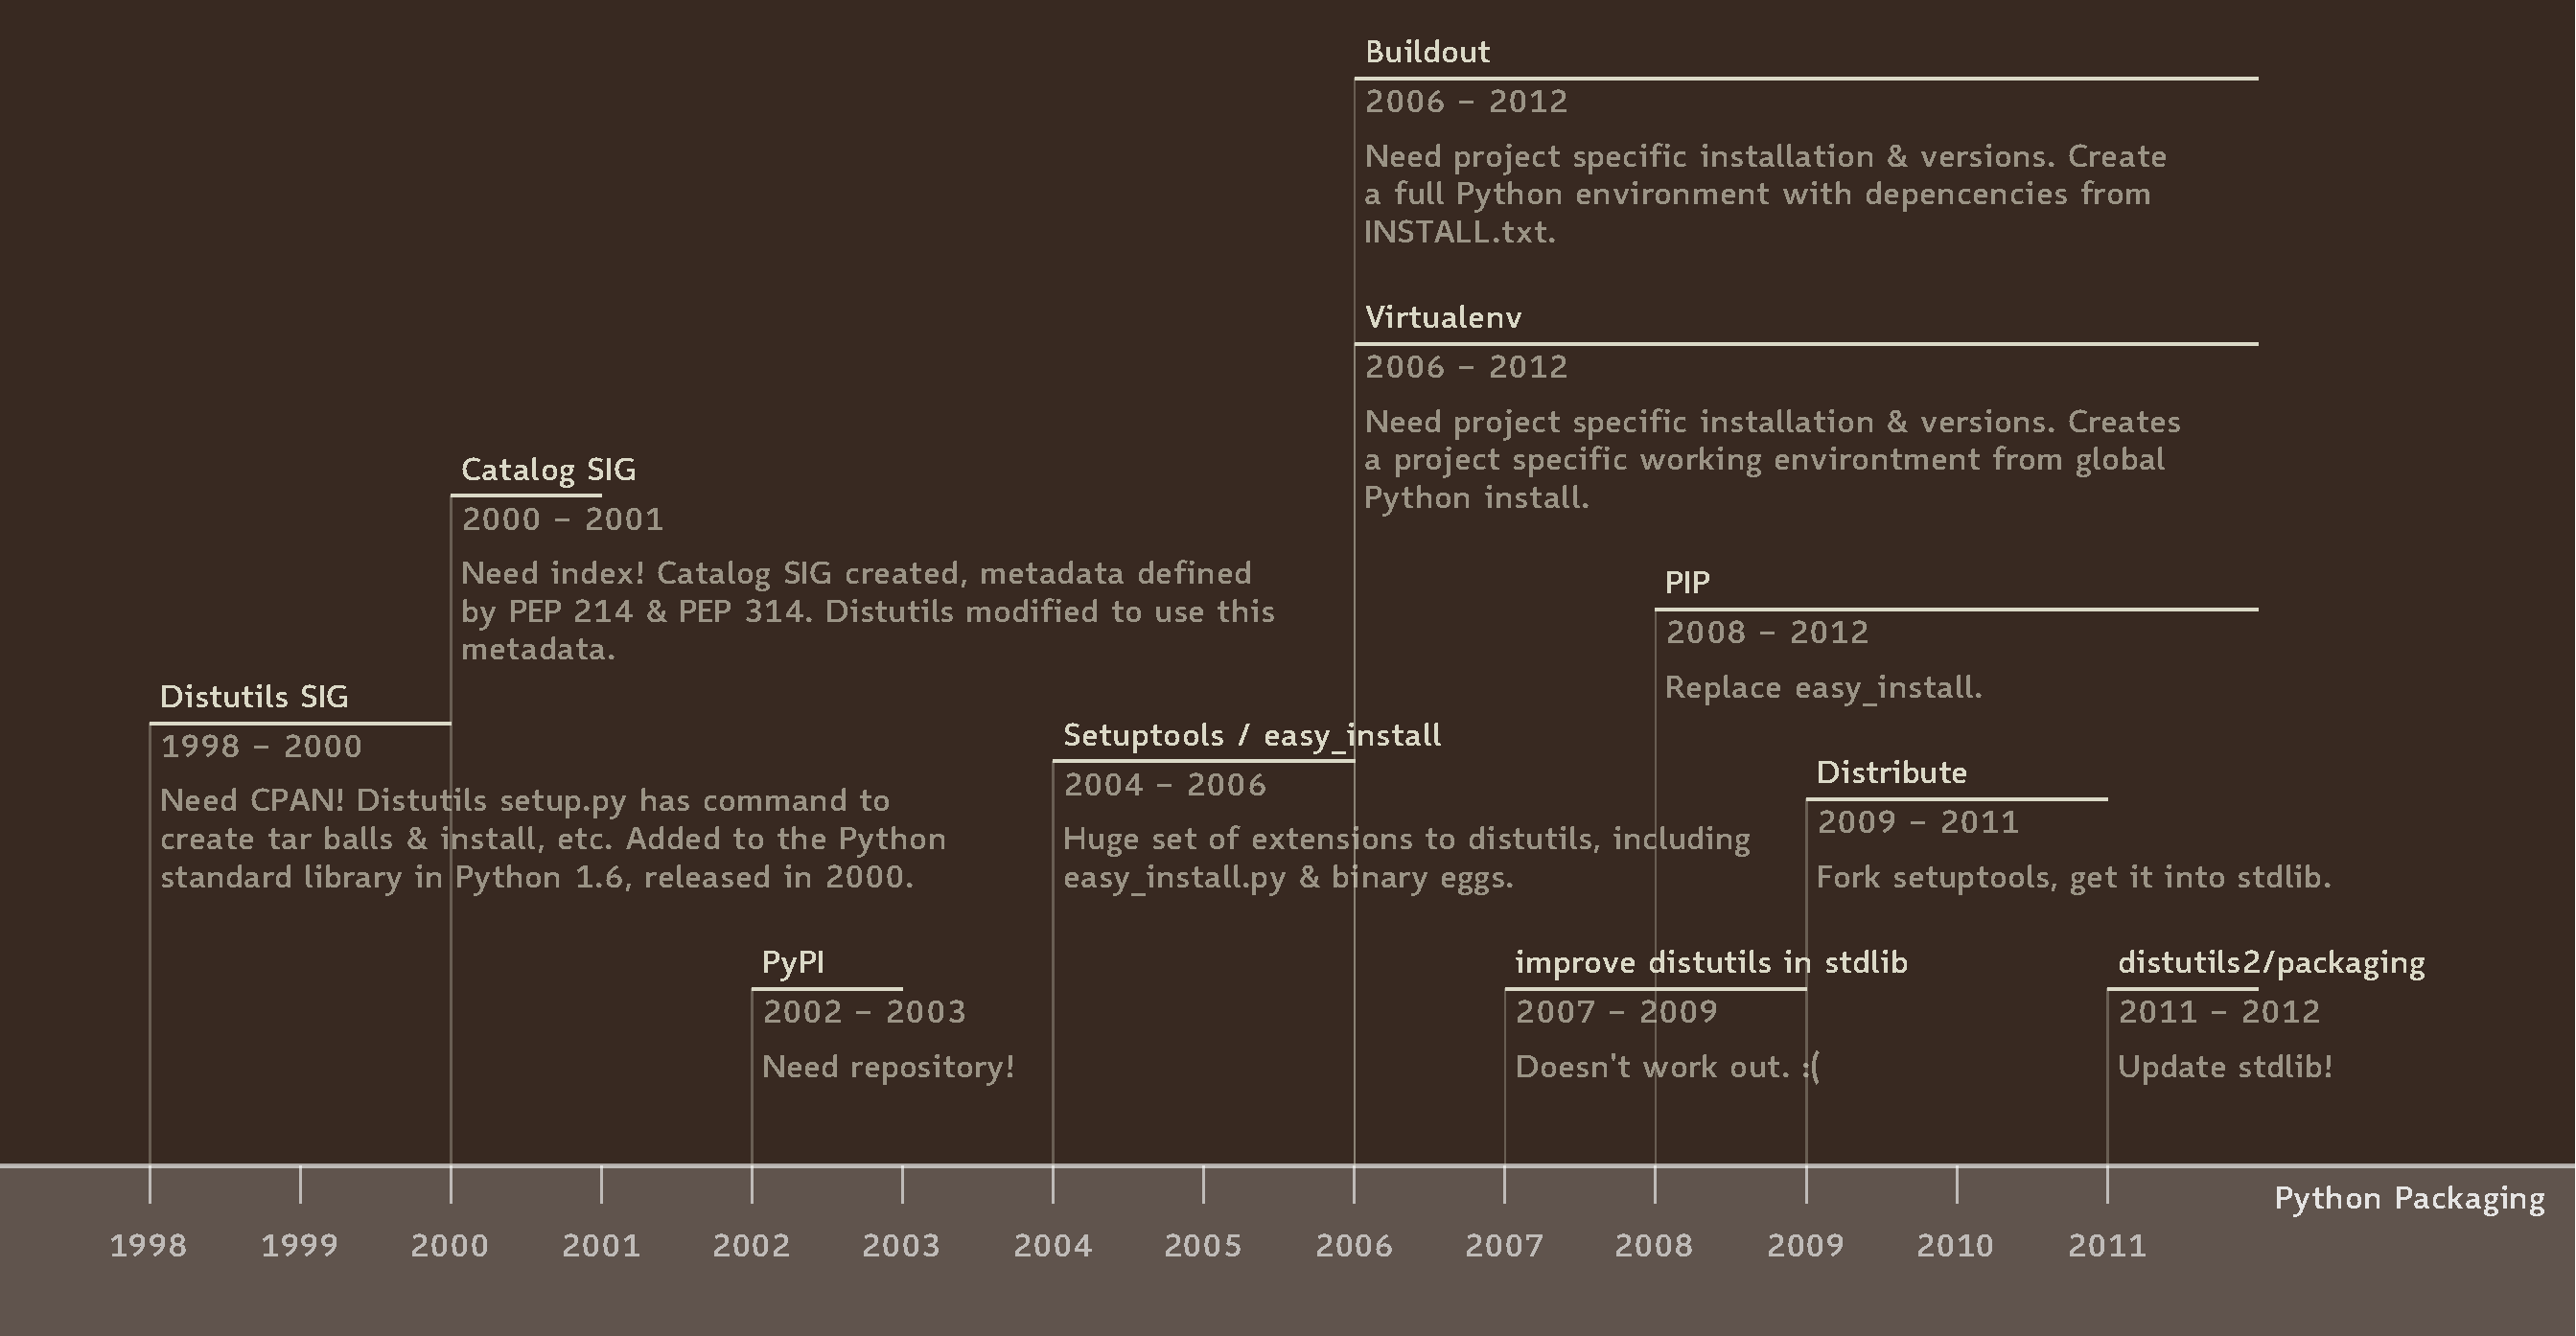
\includegraphics[width=4.5in]{PackagingTimeline.pdf}
}
\end{frame} 

% ---------------------------------------------
\begin{frame}[fragile]{Packaging Tools}

{\centering
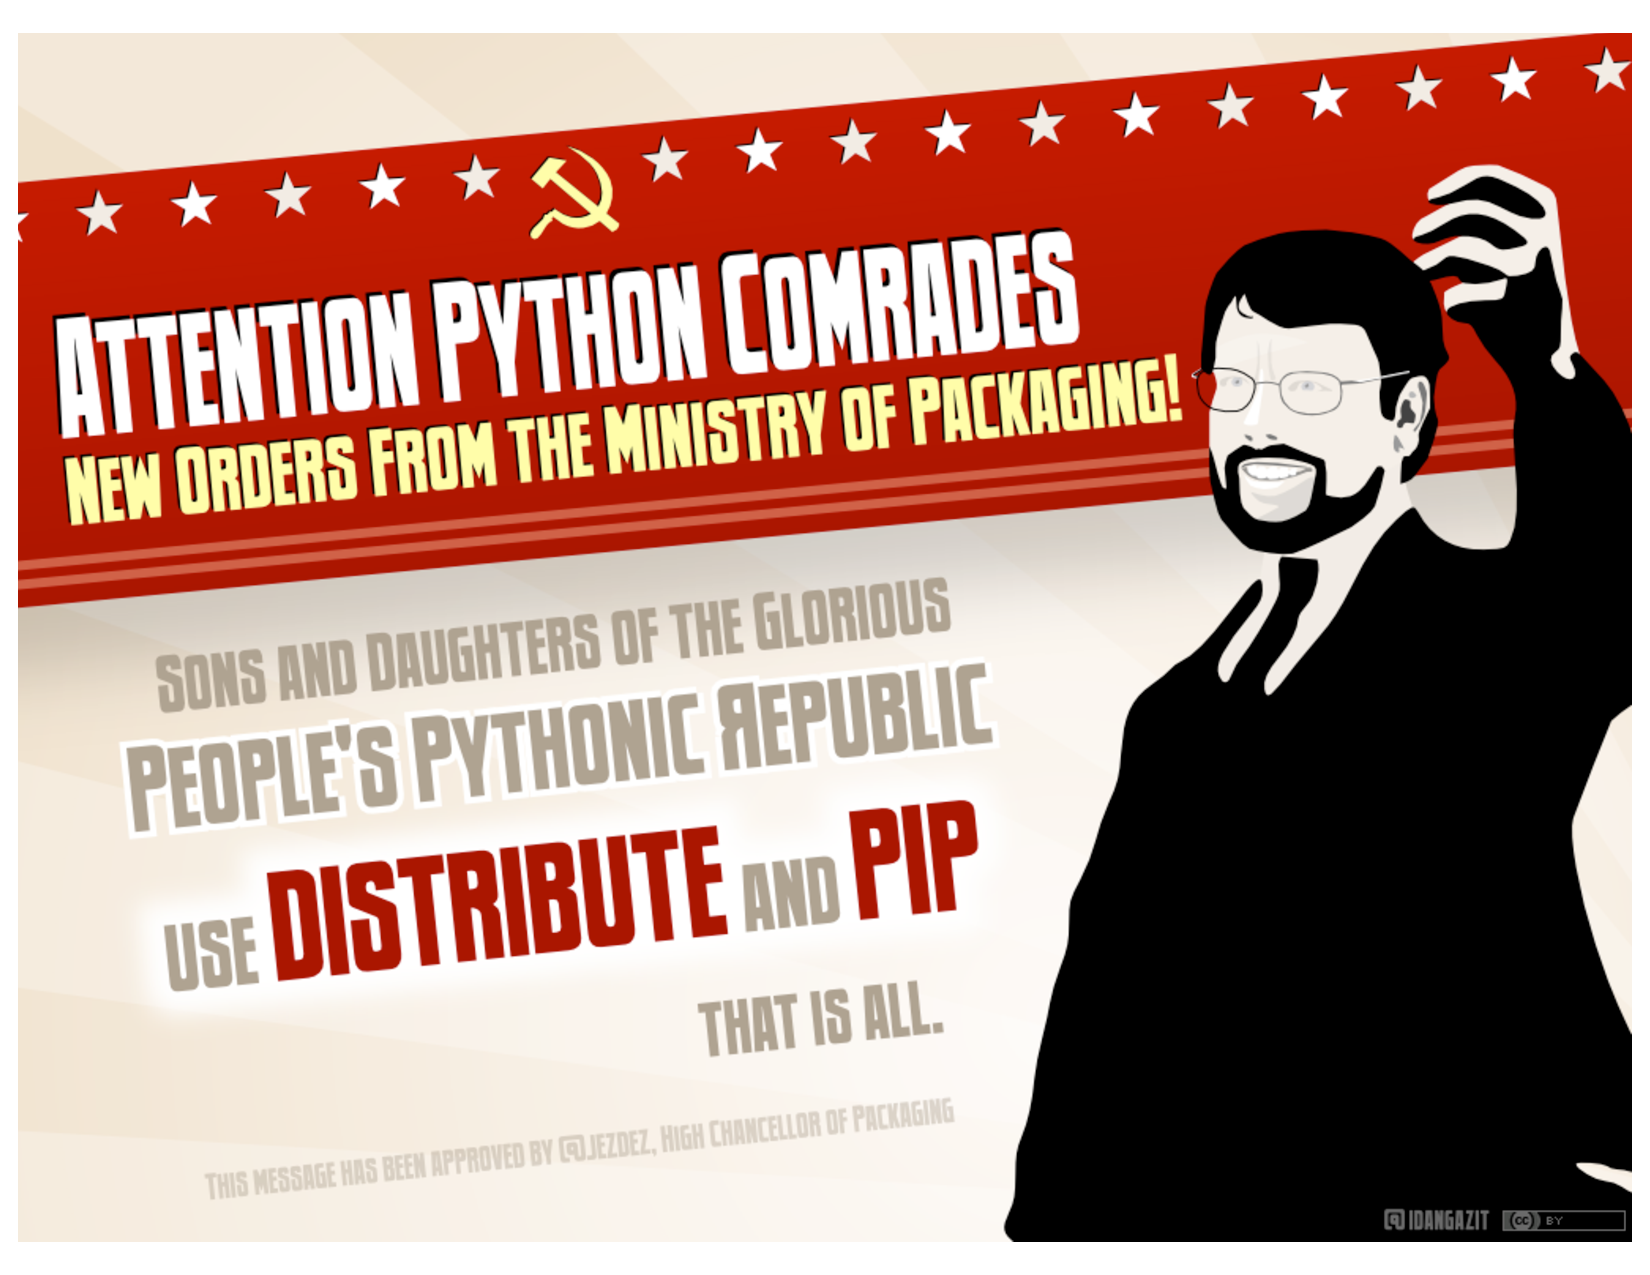
\includegraphics[width=4.5in]{packaging1.pdf}
}

\end{frame} 

% ---------------------------------------------
\begin{frame}[fragile]{Current State of Packaging}

{\centering
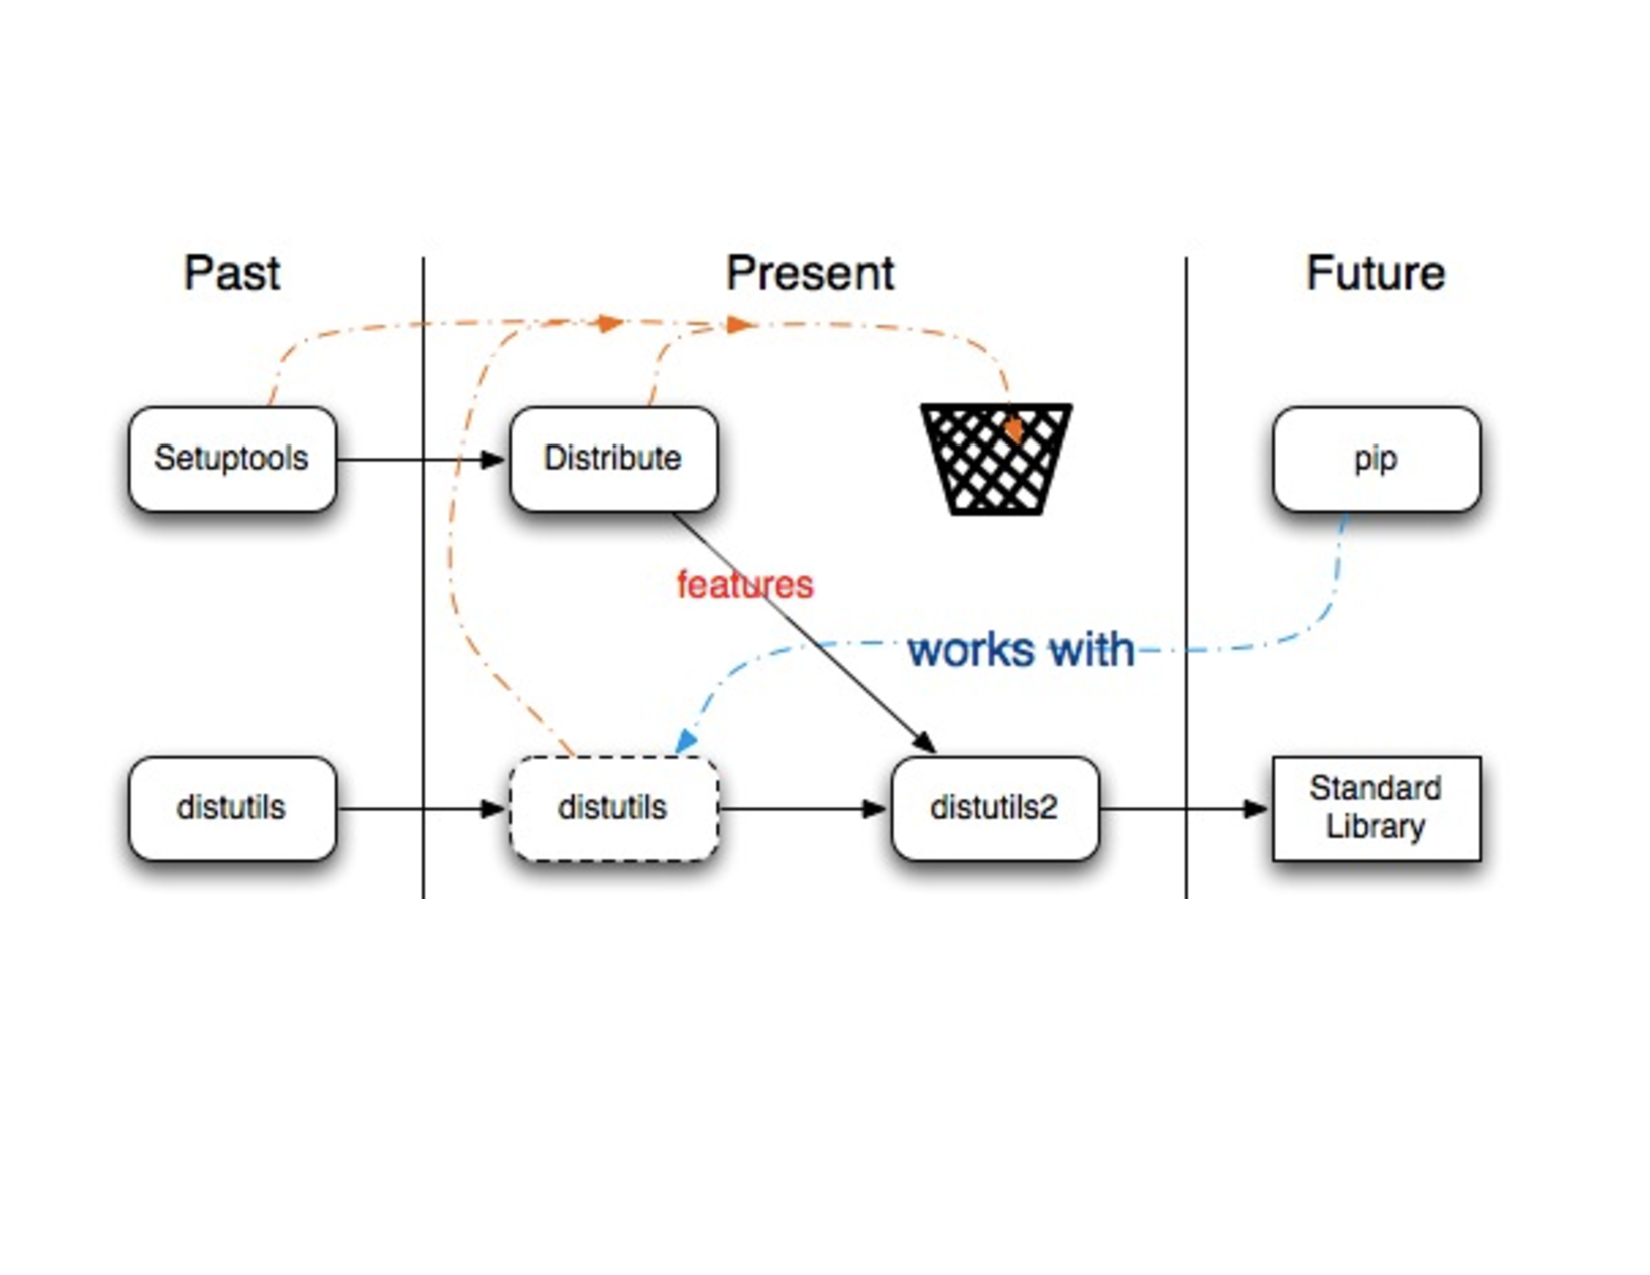
\includegraphics[width=4.5in]{PackagingCurrentState.pdf}
}
\vfill
\url{http://guide.python-distribute.org/introduction.html}
\end{frame} 

% ---------------------------------------------
\begin{frame}[fragile]{Compiled Packages}

{\LARGE Biggest issue is with compiled extensions\\[0.1in]
\hfill(C/C++, etc)\hfill
}
\vfill
{\Large -- You need the right compiler set up}

\vfill
{\LARGE Dependencies}

\vfill
{\Large -- Here's were it gets really ugly}

\vfill
{\Large -- Particularly on Windows}

\end{frame} 

% ---------------------------------------------
\begin{frame}[fragile]{Compiled Packages}

{\LARGE Linux}

\vfill
{\Large Pretty straightforward:}

\vfill
{\Large 1) Is there a system package \\[0.1in] (rpm, deb, apt-get, etc...)?
}

\vfill
{\Large 2) Install the dependencies, build from source:\\[0.1in]
\verb python setup.py build ; python setup.py install 
}

\end{frame} 

% ---------------------------------------------
\begin{frame}[fragile]{Compiled Packages}

{\LARGE Windows}

\vfill
{\Large Sometimes simpler:}

\vfill
{\Large 1) A lot of packages have Windows binaries:\\[0.1in]
            - Usually for \url{python.org} builds \\[0.1in]
            - Make sure you get 32 or 64 bit correct
}

\vfill
{\Large 2) But if no binaries: \\[0.1in]
           - Hope the dependencies are available!\\[0.1in]
           - Set up the compiler (MS "Express" version usually works)
}

\end{frame} 

% ---------------------------------------------
\begin{frame}[fragile]{Compiled Packages}

{\LARGE OS-X}

\vfill
{\Large Lots of Python versions:\\[0.1in]
  - Apple's built-in (different for each version of OS)\\[0.1in]
  - \url{python.org} builds.\\
  \hspace{0.5in}- 32 bit PPC+Intel\\
  \hspace{0.5in}- 32+64 bit Intel\\[0.1in]
  - Macports
  - Homebrew
}


\vfill
{\Large Binary Installers (dmg or egg) have to match python version}

\end{frame} 

% ---------------------------------------------
\begin{frame}[fragile]{Compiled Packages}

{\LARGE OS-X}

\vfill
{\Large If you have to build it yourself:}

\vfill
{\Large Xcode compiler (the right version:\\[0.1in]
  - Version 3.* for 32 bit PPC+Intel\\[0.1in]
  - Version 4.* for 32+64 bit Intel\\
}

\vfill
{\Large If extra dependencies:\\[0.1in]
  - macports or home brew often easiest way to build them
}

\end{frame} 

% ---------------------------------------------
\begin{frame}[fragile]{Final Recommendation}

{\Large First try: \verb|pip install|}

\vfill
{\Large If that doesn't work:}

\vfill
{\Large Read the docs of the package you want to install}

\vfill
{\Large Do what they say}

\end{frame} 

% ---------------------------------------------
\begin{frame}[fragile]{virtualenv}

{\Large \verb|virtualenv| is a tool to create isolated Python environments.}

\vfill
{\Large Very useful for developing multiple apps}

\vfill
{\Large Or deploying more than one on one system}

\vfill
\url{http://www.virtualenv.org/en/latest/index.html}
\end{frame} 

\begin{frame}[fragile]{virtualenv}

{\Large keep an eye on}

\vfill
{\Large distutils2 / packaging / pysetup }

\vfill
{\large (They are trying to solve the problem!) }

\vfill
(\url{http://packages.python.org/Distutils2/})
\end{frame} 

\section{Distributing}

\begin{frame}[fragile]{Distributing}

{\LARGE What if you need to distribute you own:}

\vfill
{\Large Scripts}

\vfill
{\large Libraries }

\vfill
{\large Applications }
\vfill

\end{frame} 

\begin{frame}[fragile]{Scripts}

\vfill
{\LARGE Often you can just copy, share, or check in the script to source
control and call it good.}

\vfill
But only if it's a single file, and doesn't need anything non-standard
\end{frame} 

\begin{frame}[fragile]{Scripts}

\vfill
{\LARGE When the script needs more than just the stdlib (or your company standard environment)}

\vfill
{\LARGE You have an application, not a script}

\vfill

\end{frame} 

\begin{frame}[fragile]{Libraries}

\vfill
{\LARGE When you read the distutils docs, it's usually libraries they’re talking about}


\vfill
{\LARGE Scripts + library is the same...}


\vfill
(\url{http://docs.python.org/distutils/})
\end{frame} 

\begin{frame}[fragile]{distutils}

\vfill
{\LARGE \verb|distutils| makes it easy to do the easy stuff:}

\vfill
{\Large Distribute and install to multiple platforms, etc.}

\vfill
{\Large Even binaries, installers and compiled packages}

\vfill
{\Large (Except dependencies)}

\vfill
(\url{http://docs.python.org/distutils/})
\end{frame} 

\begin{frame}[fragile]{distutils basics}

\vfill
{\Large It's all in the \verb|setup.py file|:}

\begin{verbatim}
from distutils.core import setup
setup(name='Distutils',
      version='1.0',
      description='Python Distribution Utilities',
      author='Greg Ward',
      author_email='gward@python.net',
      url='http://www.python.org/sigs/distutils-sig/',
      packages=['distutils', 'distutils.command'],
     )
\end{verbatim}
\vfill
(\url{http://docs.python.org/distutils/})
\end{frame} 

\begin{frame}[fragile]{distutils basics}

{\Large Once your setup.py is written, you can:}

\begin{verbatim}
python setup.py ...

build         build everything needed to install
install       install everything from build directory
sdist         create a source distribution
              (tarball, zip file, etc.)
bdist         create a built (binary) distribution
bdist_rpm     create an RPM distribution
bdist_wininst create an executable installer for MS Windows
upload        upload binary package to PyPI
\end{verbatim}

\end{frame} 

%----------------------------------------------
\begin{frame}[fragile]{More complex packaging}

{\Large For a complex package:}

\vfill
{\Large You want to use a well structured setup:}

\vfill
\url{http://guide.python-distribute.org/creation.html}
\vfill
\end{frame} 

%----------------------------------------------
\begin{frame}[fragile]{develop mode}

{\Large While you are developing your package, Installing it is a pain.}

\vfill
{\Large But you want your code to be able to import, etc. as though it were installed}

\vfill
{\Large \verb|setup.py develop| installs links to your code, rather than copies
 -- so it looks like it's installed, but it's using the original source}

\vfill
{\Large You need \verb|distribute| (or \verb|setuptools|) to use it.}
\vfill
\end{frame} 

%----------------------------------------------
\begin{frame}[fragile]{Applications}

{\Large For a complete application:}
\begin{itemize}
  \item Web apps
  \item GUI apps
\end{itemize}

{\Large Multiple options:}
\begin{itemize}
  \item Virtualenv + VCS
  \item zc.buildout ( \url{http://www.buildout.org/} )
  \item System packages (rpm, deb, ...)
  \item Bundles...
\end{itemize}

\end{frame} 

%----------------------------------------------
\begin{frame}[fragile]{Bundles}

{\Large
Bundles are Python + all your code + plus all the dependencies --
all in one single ``bundle'' 

\vfill
Most popular on Windows and OS-X
}
\begin{verbatim}
  py2exe
  py2app
  pyinstaller
 ...
\end{verbatim}

{\Large User doesn't even have to know it's python }

\vfill
Examples: \\
\hspace{0.5in} \url{http://www.bitpim.org/} \\
\hspace{0.5in} \url{http://response.restoration.noaa.gov/nucos}

\end{frame} 


%-------------------------------
\begin{frame}[fragile]{LAB}

{\Large Write a setup.py for a script of yours}

\begin{itemize}
  \item Ideally, your script relies on at least one other module
  \item At a minimum, you'll need to specify \verb|scripts|
  \item and probably \verb|py_modules|
  \item try:
  \begin{itemize}
    \item \verb| python setup.py build| 
    \item \verb| python setup.py install| 
    \item \verb| python setup.py sdist| 
    \item \verb| python setup.py bdist_wininst| 
  \end{itemize}
  \item EXTRA: install \verb|distribute|
  \begin{itemize}
    \item use: \verb|from setuptools import setup|
    \item try: \verb| python setup.py develop| 
  \end{itemize}
\end{itemize}

\end{frame}

%%-------------------------------
%\begin{frame}{Wrap up}
%
%\begin{itemize}
%  \item decorators
%  \item 
%  \item decorators
%\end{itemize}
%
%\end{frame}
%


%-------------------------------
\begin{frame}{Homework}

\begin{itemize}
  \item Find a package or two and install it
  \item Try to install it "from source" -- i.e. \verb|setup.py install| 
  \itme Make a nice package of your class project (or something else)
\end{itemize}

\end{frame}


\end{document}

 
